\documentclass[journal,12pt,twocolumn]{IEEEtran}
%
\usepackage{setspace}
\usepackage{gensymb}
%\doublespacing
\singlespacing

%\usepackage{graphicx}
%\usepackage{amssymb}
%\usepackage{relsize}
\usepackage[cmex10]{amsmath}
%\usepackage{amsthm}
%\interdisplaylinepenalty=2500
%\savesymbol{iint}
%\usepackage{txfonts}
%\restoresymbol{TXF}{iint}
%\usepackage{wasysym}
\usepackage{amsthm}
%\usepackage{iithtlc}
\usepackage{mathrsfs}
\usepackage{txfonts}
\usepackage{stfloats}
\usepackage{bm}
\usepackage{cite}
\usepackage{cases}
\usepackage{subfig}
%\usepackage{xtab}
\usepackage{longtable}
\usepackage{multirow}
%\usepackage{algorithm}
%\usepackage{algpseudocode}
\usepackage{enumitem}
\usepackage{mathtools}
\usepackage{steinmetz}
\usepackage{tikz}
\usepackage{circuitikz}
\usepackage{verbatim}
\usepackage{tfrupee}
\usepackage[breaklinks=true]{hyperref}
%\usepackage{stmaryrd}
\usepackage{tkz-euclide} % loads  TikZ and tkz-base
%\usetkzobj{all}
\usetikzlibrary{calc,math}
\usepackage{listings}
    \usepackage{color}                                            %%
    \usepackage{array}                                            %%
    \usepackage{longtable}                                        %%
    \usepackage{calc}                                             %%
    \usepackage{multirow}                                         %%
    \usepackage{hhline}                                           %%
    \usepackage{ifthen}                                           %%
  %optionally (for landscape tables embedded in another document): %%
    \usepackage{lscape}     
\usepackage{multicol}
\usepackage{chngcntr}
%\usepackage{enumerate}
\usepackage{hyperref}
%\usepackage{wasysym}
%\newcounter{MYtempeqncnt}
\DeclareMathOperator*{\Res}{Res}
%\renewcommand{\baselinestretch}{2}
\renewcommand\thesection{\arabic{section}}
\renewcommand\thesubsection{\thesection.\arabic{subsection}}
\renewcommand\thesubsubsection{\thesubsection.\arabic{subsubsection}}

\renewcommand\thesectiondis{\arabic{section}}
\renewcommand\thesubsectiondis{\thesectiondis.\arabic{subsection}}
\renewcommand\thesubsubsectiondis{\thesubsectiondis.\arabic{subsubsection}}

% correct bad hyphenation here
\hyphenation{op-tical net-works semi-conduc-tor}
\def\inputGnumericTable{}                                 %%

\lstset{
%language=C,
frame=single, 
breaklines=true,
columns=fullflexible
}
%\lstset{
%language=tex,
%frame=single, 
%breaklines=true
%}

\begin{document}
%


\newtheorem{theorem}{Theorem}[section]
\newtheorem{problem}{Problem}
\newtheorem{proposition}{Proposition}[section]
\newtheorem{lemma}{Lemma}[section]
\newtheorem{corollary}[theorem]{Corollary}
\newtheorem{example}{Example}[section]
\newtheorem{definition}[problem]{Definition}
%\newtheorem{thm}{Theorem}[section] 
%\newtheorem{defn}[thm]{Definition}
%\newtheorem{algorithm}{Algorithm}[section]
%\newtheorem{cor}{Corollary}
\newcommand{\BEQA}{\begin{eqnarray}}
\newcommand{\EEQA}{\end{eqnarray}}
\newcommand{\define}{\stackrel{\triangle}{=}}

\bibliographystyle{IEEEtran}
%\bibliographystyle{ieeetr}


\providecommand{\mbf}{\mathbf}
\providecommand{\pr}[1]{\ensuremath{\Pr\left(#1\right)}}
\providecommand{\qfunc}[1]{\ensuremath{Q\left(#1\right)}}
\providecommand{\sbrak}[1]{\ensuremath{{}\left[#1\right]}}
\providecommand{\lsbrak}[1]{\ensuremath{{}\left[#1\right.}}
\providecommand{\rsbrak}[1]{\ensuremath{{}\left.#1\right]}}
\providecommand{\brak}[1]{\ensuremath{\left(#1\right)}}
\providecommand{\lbrak}[1]{\ensuremath{\left(#1\right.}}
\providecommand{\rbrak}[1]{\ensuremath{\left.#1\right)}}
\providecommand{\cbrak}[1]{\ensuremath{\left\{#1\right\}}}
\providecommand{\lcbrak}[1]{\ensuremath{\left\{#1\right.}}
\providecommand{\rcbrak}[1]{\ensuremath{\left.#1\right\}}}
\theoremstyle{remark}
\newtheorem{rem}{Remark}
\newcommand{\sgn}{\mathop{\mathrm{sgn}}}
\providecommand{\abs}[1]{\left\vert#1\right\vert}
\providecommand{\res}[1]{\Res\displaylimits_{#1}} 
\providecommand{\norm}[1]{\left\lVert#1\right\rVert}
%\providecommand{\norm}[1]{\lVert#1\rVert}
\providecommand{\mtx}[1]{\mathbf{#1}}
\providecommand{\mean}[1]{E\left[ #1 \right]}
\providecommand{\fourier}{\overset{\mathcal{F}}{ \rightleftharpoons}}
%\providecommand{\hilbert}{\overset{\mathcal{H}}{ \rightleftharpoons}}
\providecommand{\system}{\overset{\mathcal{H}}{ \longleftrightarrow}}
	%\newcommand{\solution}[2]{\textbf{Solution:}{#1}}
\newcommand{\solution}{\noindent \textbf{Solution: }}
\newcommand{\cosec}{\,\text{cosec}\,}
\providecommand{\dec}[2]{\ensuremath{\overset{#1}{\underset{#2}{\gtrless}}}}
\newcommand{\myvec}[1]{\ensuremath{\begin{pmatrix}#1\end{pmatrix}}}
\newcommand{\mydet}[1]{\ensuremath{\begin{vmatrix}#1\end{vmatrix}}}
%\numberwithin{equation}{section}
\numberwithin{equation}{subsection}
%\numberwithin{problem}{section}
%\numberwithin{definition}{section}
\makeatletter
\@addtoreset{figure}{problem}
\makeatother

\let\StandardTheFigure\thefigure
\let\vec\mathbf
%\renewcommand{\thefigure}{\theproblem.\arabic{figure}}
\renewcommand{\thefigure}{\theproblem}
%\setlist[enumerate,1]{before=\renewcommand\theequation{\theenumi.\arabic{equation}}
%\counterwithin{equation}{enumi}


%\renewcommand{\theequation}{\arabic{subsection}.\arabic{equation}}

\def\putbox#1#2#3{\makebox[0in][l]{\makebox[#1][l]{}\raisebox{\baselineskip}[0in][0in]{\raisebox{#2}[0in][0in]{#3}}}}
     \def\rightbox#1{\makebox[0in][r]{#1}}
     \def\centbox#1{\makebox[0in]{#1}}
     \def\topbox#1{\raisebox{-\baselineskip}[0in][0in]{#1}}
     \def\midbox#1{\raisebox{-0.5\baselineskip}[0in][0in]{#1}}

\vspace{3cm}


\title{PT100 Experiment using Gradient Descent}
\author{Nikam Pratik Balasaheb (EE21BTECH11037)}





% make the title area
\maketitle

\newpage

%\tableofcontents

\bigskip

\renewcommand{\thefigure}{\theenumi}
\renewcommand{\thetable}{\theenumi}
%\renewcommand{\theequation}{\theenumi}

\begin{abstract}
	The volatge readings from Voltage divider having PT100 sensor one of the arms is mapped to corresponding temperatue. \texttt{numpy.linalg.lstsq} was initially used to fit a linear curve over data.
	Refer \href{https://github.com/N-Pratik/EE2802/tree/main/PT100}{PT100 experiment}.\\
	Now, Gradient Descent method is used to obtain the parameters of linear relation.
\end{abstract}

\section{Cost Function}

Here, cost function or error function is defined as mean of squared errors.i.e.
\begin{align}
	Cost(\vec{n}) &= \frac{1}{m}\sum_{i=1}^{m} (y_i - \hat{y}_i)^2 \\
	&= \frac{1}{m} \brak{ \vec{X}\vec{n} - \vec{y} }^T \brak{ \vec{X}\vec{n} - \vec{y} }
\end{align}
where $y_i$ is the actual value and $\hat{y}_i$ is the predicted value and $m$ is the number of data points.\\
$\vec{n}$ is the vector of parameters of linear relation.\\
\begin{align}
	\vec{n} = \myvec{A\\B}
\end{align}
The plot of cost function with respect to $A$ and $B$ is shown in figure \ref{fig:cost}.

\begin{figure}[h!]
  \centering
   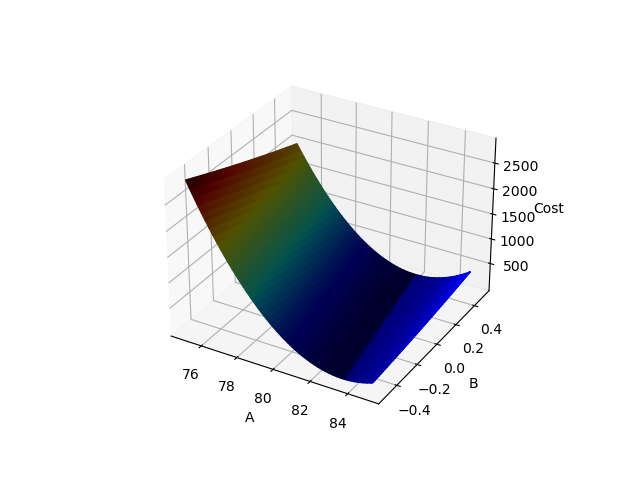
\includegraphics[width=\linewidth]{figs/cost.png}
   \caption{Cost}
   \label{fig:cost}
\end{figure}

\texttt{codes/cost.py} contains the code for plotting the cost function.

\section{Method}

For minimizing the cost function, gradient descent method is used.\\
The gradient of cost function is given by:
\begin{align}
	\frac{\partial{Cost}}{\partial{n}} = \frac{1}{m}\sum_{i=1}^{m} 2(y_i - \hat{y}_i) \frac{\partial{\hat{y}_i}}{\partial{n}}\\
	= \frac{2}{m} \brak{ \vec{X}\vec{n} - \vec{y} }^T \vec{X}
\end{align}

The parameters are updated as,
\begin{align}
	\vec{n} = \vec{n} - \alpha \frac{\partial{Cost}}{\partial{n}}
\end{align}

where $\alpha$ is the learning rate.\\
Above equation is run on loop until the cost function is lesser than a certain tolerance.

\section{Results}
	Above method is implemented in \texttt{codes/Grad\_Des.py}
	with tolerance of 1 and Learning rate of $4.72 \times 10^{-5}$\\
	
	\begin{table}[h!]
	\centering
	       

	       \caption{Data used for training}
	       \label{tab:Train_data}
	\end{table}

	The data used for training the model is given in Table \ref{tab:Train_data}.
	Resulting parameters:
	\begin{align}
		n = \myvec{78.37174146 \\ 0.28238033}
	\end{align}

	\begin{figure}[h!]
	  \centering
	   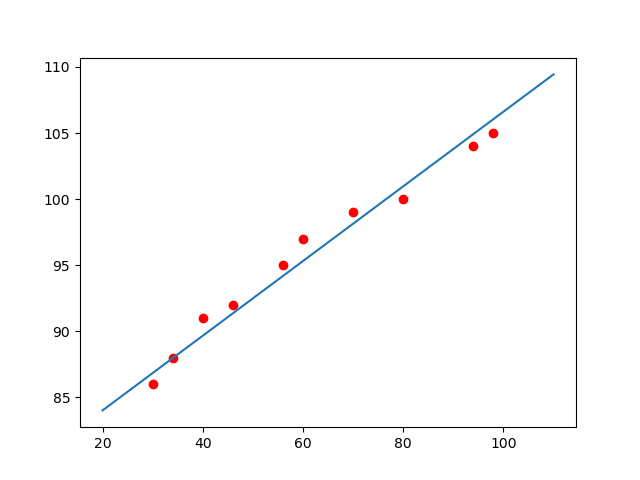
\includegraphics[width=\linewidth]{figs/Training_GD.png}
	   \caption{Training}	\label{fig:Train}
	\end{figure}
	
	The plot of training data and predicted line is shown in figure \ref{fig:Train}.

\section{Testing}
	The model is used to predict the results for the test data.
	\begin{table}[h!]
        \centering 
               %%%%%%%%%%%%%%%%%%%%%%%%%%%%%%%%%%%%%%%%%%%%%%%%%%%%%%%%%%%%%%%%%%%%%%
%%                                                                  %%
%%  This is a LaTeX2e table fragment exported from Gnumeric.        %%
%%                                                                  %%
%%%%%%%%%%%%%%%%%%%%%%%%%%%%%%%%%%%%%%%%%%%%%%%%%%%%%%%%%%%%%%%%%%%%%%

\begin{tabular}[]{|c|c|}
\hline
Temperature	& Reading	\\ \hline
  31  & 87  \\ \hline
  52  & 94  \\ \hline
  66  & 98  \\ \hline
  90  & 103  \\ \hline
\end{tabular}
               \caption{Data used for testing}    
               \label{tab:Test_data}
        \end{table}

	The data used for testing in given in Table \ref{tab:Test_data}
	
	\begin{figure}[h!]
	  \centering
	   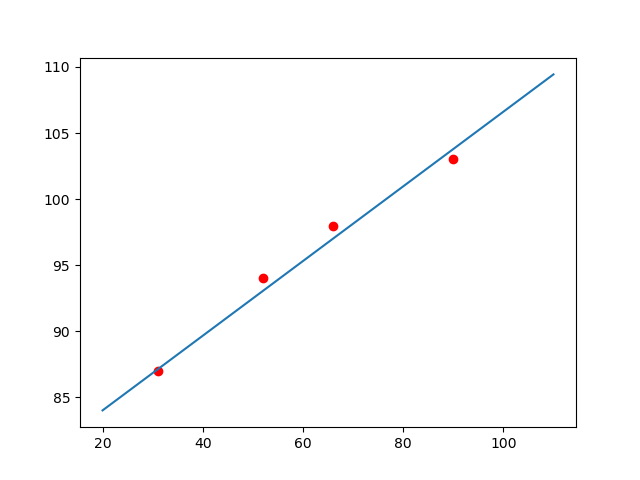
\includegraphics[width=\linewidth]{figs/Test_GD.png}
	   \caption{Testing}
	   \label{fig:Test}
	\end{figure}

	The plot of test data and predicted line is shown in figure \ref{fig:Test}.

	Mean Squared Error in Testing = 0.62699
%\begin{figure}[h!]
%  \centering
%   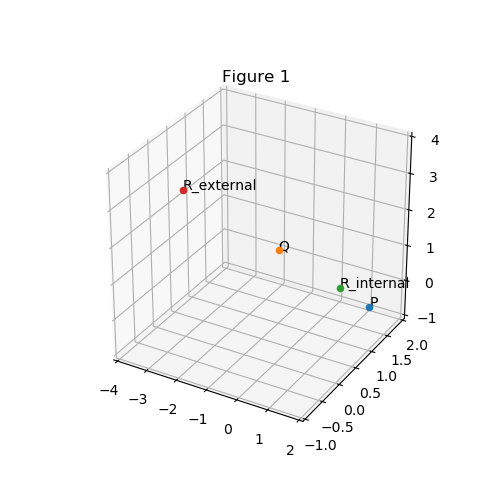
\includegraphics[width=\linewidth]{figs/Figure_1.png}
%   \caption{Figure}
%   \label{fig:}
%\end{figure}

%\begin{table}
%\centering
%	%%%%%%%%%%%%%%%%%%%%%%%%%%%%%%%%%%%%%%%%%%%%%%%%%%%%%%%%%%%%%%%%%%%%%%
%%                                                                  %%
%%  This is a LaTeX2e table fragment exported from Gnumeric.        %%
%%                                                                  %%
%%%%%%%%%%%%%%%%%%%%%%%%%%%%%%%%%%%%%%%%%%%%%%%%%%%%%%%%%%%%%%%%%%%%%%

\begin{tabular}[]{|c|c|c|}
\hline
Parameter	& Value		& Description\\ \hline
$\vec{O}$	& $\myvec{5\\0}$ &Center of the given circle \\ \hline
$\vec{B}$	& $\myvec{0\\0}$ &Point where Salma is standing\\ \hline
$r$		& 5 & radius of given circle \\ \hline
$d$ 		& 6 & distance AB and BC\\ \hline
\end{tabular}

%	\caption{Table}
%	\label{tab:}
%\end{table}

\end{document}



